% Shared standalone design for the editable figure reconstructions.
\documentclass[tikz,border=5pt,10pt]{standalone}
\usepackage[T1]{fontenc}
\usepackage[utf8]{inputenc}
\usepackage{newpxtext,newpxmath}
\usepackage[scaled=.94]{sourcesanspro}
\usepackage{pgfplots}
\pgfplotsset{compat=1.18}
\usetikzlibrary{arrows.meta,calc,positioning,decorations.pathreplacing,
  decorations.markings,patterns,matrix,shapes.geometric,fit,backgrounds,
  intersections,angles,quotes}
\definecolor{ink}{HTML}{203746}
\definecolor{accent}{HTML}{146C78}
\definecolor{muted}{HTML}{667780}
\definecolor{signalred}{HTML}{B94B44}
\color{ink}
\tikzset{>=Latex,line width=.8pt,
  every node/.style={font=\small},
  axis/.style={->,draw=muted,line width=.5pt},
  guide/.style={draw=muted,dashed,line width=.45pt},
  curve/.style={draw=accent,line width=1pt},
  marker/.style={circle,fill=accent,inner sep=1.5pt},
  labelbox/.style={fill=white,inner sep=2pt}}


\begin{document}
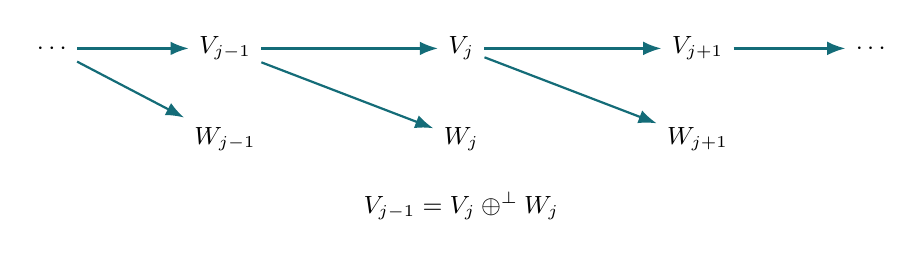
\begin{tikzpicture}[>=Latex,line width=.8pt]
\node (v0) at (2,0) {$V_{j-1}$};
\node (w0) at (2,-1.15) {$W_{j-1}$};
\node (v1) at (5,0) {$V_{j}$};
\node (w1) at (5,-1.15) {$W_{j}$};
\node (v2) at (8,0) {$V_{j+1}$};
\node (w2) at (8,-1.15) {$W_{j+1}$};
\node (left) at (-.2,0) {$\cdots$};\node (right) at (10.2,0) {$\cdots$};
\draw[->,accent] (left)--(v0);\draw[->,accent] (v0)--(v1);\draw[->,accent] (v1)--(v2);\draw[->,accent] (v2)--(right);
\draw[->,accent] (left)--(w0);\draw[->,accent] (v0)--(w1);\draw[->,accent] (v1)--(w2);
\node[align=center] at (5,-2) {$V_{j-1}=V_j\mathbin{\oplus^{\perp}}W_j$};
\end{tikzpicture}
\end{document}
